% Chapter 2 Support Vector Machine

\chapter{پشینیه پژوهش} \label{ch:2}
\section{ماشین بردار پشتیبان} \label{sec:2:1}
در این بخش، ابتدا ماشین بردار پشتیبان خطی و غیر خطی شرح داده می‌شود. سپس پیشینه پژوهش در زمینه ماشین بردار پشتیبان بررسی می‌گردد.
\subsection{ماشین بردار پشتیبان با حاشیه سخت} \label{sec:2:1:1}
ماشین بردار پشتیبان با هدف جداسازی نمونه‌های دو کلاس در سال 1995 معرفی گردید \cite{vapnik1995}. ایده اصلی این روش یادگیری، بدست آوردن ابرصفحه بهینه‌ای است که از نمونه‌های دو کلاس تا جای ممکن بیشترین فاصله را داشته باشد. به عبارت دیگر، این روش یادگیری حاشیه دو کلاس را بیشینه می‌کند. برای فهم بهتر ایده این روش، فرض کنید مجموعه داده‌ی $T=\{(x_1, y_1),(x_2, y_2) \cdots , (x_m, y_m)\}$ را در اختیار داریم که شامل $m$ تا نمونه آموزشی است. هر نمونه آموزشی $x_{i} \in \mathbb{R}^{n}$ با $n$ ویژگی در فضای ورودی و $y_i \in \{-1,1\}$ برچسب نمونه‌ی $x_i$ می‌باشد. در ساده‌ترین حالت، نمونه‌های دو کلاس در مجموعه داده $T$ با یک ابرصفحه $w^{T}x+b$ بدون خطا دسته‌بندی می‌شود. این حالت مسئله حاشیه سخت\footnote{\lr{Hard margin}}  نامیده می‌شود. شکل \ref{fig:SVM-HM} مسئله حاشیه سخت در روش \lr{SVM} را نشان می‌دهد. (لازم به ذکر است، خطوط نقطه‌چین در شکل ‏\ref{fig:SVM-HM} نشان دهنده حاشیه است.) در این حالت، یک مسئله بهینه‌سازی برای بدست آوردن ابرصفحه باید حل گردد.

\begin{equation}
\begin{gathered} 
\mathop{min}\limits_{w}\frac{1}{2}{{\left\| w \right\|}^{2}} \\
\textrm{\lr{s.t. }} {{y}_{i}}({{w}^T}{{x}_{i}}+b)\ge 1,\forall i
\end{gathered}
\label{eq:1}
\end{equation}

\begin{figure}[!t]
	\centering
	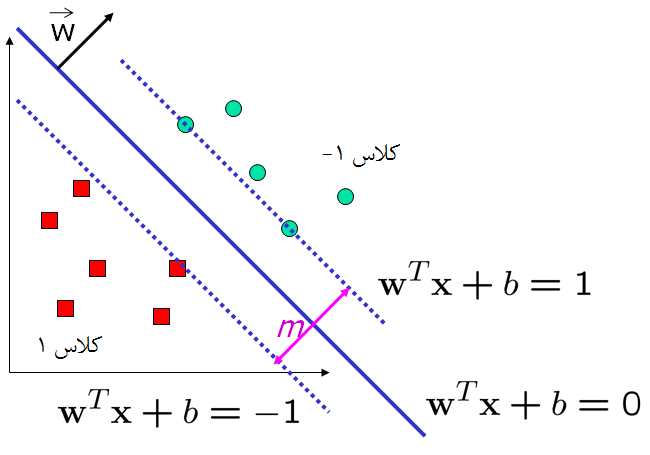
\includegraphics[scale=0.5]{SVM-HardMargin}
	\caption{مسئله حاشیه سخت در ماشین بردار پشتیبان}
	\label{fig:SVM-HM}
\end{figure}

\noindent در رابطه \ref{eq:1}، بردار $w$ مختصات ابرصفحه و $b$ بایاس است. قید این مسئله بهنیه‌سازی بیان می‌کند که تمام نمونه‌های آموزشی باید از ابرصفحه به مقدار 1 یا بیشتر فاصله داشته باشند. به عبارت دیگر، تمام نمونه‌های آموزشی باید روی خط حاشیه یا قبل از آن قرار بگیرند. برای حل کردن مسئله بهینه‌سازی \ref{eq:1} از تابع لاگرانژ\footnote{\lr{Lagrange}}  استفاده می‌شود که در رابطه زیر تعریف شده است. 
\begin{equation}
L(w,b,\alpha )=\frac{1}{2}{{\left\| w \right\|}^{2}}-\sum\limits_{i=1}^{m}{{{\alpha }_{i}}({{y}_{i}}({{w}^{T}}{{x}_{i}}+b)-1})
\label{eq:2}
\end{equation} 
در رابطه \ref{eq:2}، بردار $\alpha$ نشان دهنده ضرایب لاگرانژ است. برای حل کردن رابطه \ref{eq:2}، از تابع لاگرانژ نسبت به $w$ و  $b$ مشتق می‌گیریم.
\begin{align}
\label{eq:3}
\begin{split}
\frac{\partial L}{\partial b}=0&\quad \Rightarrow \quad \sum\limits_{i=1}^{m}{{{\alpha }_{i}}{{y}_{i}}}=0 
\end{split}\\ 
\label{eq:4}
\begin{split}
\frac{\partial L}{\partial w}=0& \quad \Rightarrow \quad w = \sum\limits_{i=1}^{m}{\alpha_{i}y_{i}x_{i}}. 
\end{split} 
\end{align}

با استفاده از اصل دوگانگی لاگرانژ، مسئله اصلی\footnote{\lr{Primal problem}}  در رابطه \ref{eq:1} می‌تواند به مسئله دوگان\footnote{\lr{Dual problem}}  تبدیل شود که حل کردن آن آسان‌تر از مسئله اصلی خواهد بود. با در نظر گرفتن روابط \ref{eq:3} و \ref{eq:4}، مسئله دوگان برای حالت حاشیه سخت به صورت زیر تعریف می‌شود.
\begin{equation}
\begin{split} 
\min\limits_{\alpha} \quad &\frac{1}{2}\sum\limits_{i=1}^{m}{\sum\limits_{j=1}^{m}{{{\alpha }_{i}}{{\alpha }_{j}}{{y}_{i}}{{y}_{j}}x_{i}^{T}{{x}_{j}}-\sum\limits_{k=1}^{m}{{{\alpha }_{k}}}}} \\
\textrm{\lr{s.t. }} \quad &\sum\limits_{i=1}^{m}{\alpha_{i}y_{i}}=0, \\
&\alpha_{i}\ge 0,\text{ }\forall i
\end{split}
\label{eq:5}
\end{equation}
بعد از حل کردن مسئله دوگان \ref{eq:5}، اکثر مقادیر بردار $\alpha$ برابر با صفر خواهد. با این حال ضرایب لاگرانژ  $\alpha_i$ متناظر با نمونه‌های $x_i$ بزرگتر از صفر خواهد بود، اگر معادله زیر برقرار باشد.
\begin{equation}
{{y}_{i}}({{w}^{T}}{{x}_{i}}+b)=1
\label{eq:6}
\end{equation}
\indent نمونه‌های  که رابطه \ref{eq:6} برای آن‌ها برقرار باشد، به اصطلاح بردار پشتیبان\footnote{\lr{Suppor Vector (SV)}}  نامیده می‌شود. ضرایب لاگرانژ متناظر با بردار‌های پشتیبان بزرگ‌تر از صفر است. همچنین این بردارها روی حاشیه قرار می‌گیرند. بردار $w$  و بایاس  $b$ از طریق رابطه  بدست می‌آید.
\begin{equation}
\begin{split}
w &= \sum\limits_{i=1}^{m}{\alpha_{i}y_{i}x_{i}} \\
b &= y_{i}-{w}^{T}{x}_{i}
\end{split}
\label{eq:7}
\end{equation}
یک نمونه جدید یا تست بر اساس تابع تصمیم در رابطه زیر به یکی از کلاس‌های 1 و 1- تعلق می‌گیرد.
\begin{equation}
D(x)=sign({{w}^{T}}x+b) = sign(\sum\limits_{i=1}^{m}{\alpha_{i}y_{i}x_{i}^{T}} x + b)
\label{eq:8}
\end{equation}
\indent در مسئله حاشیه سخت، فرض گرفته می‌شود که تمام نمونه‌های دو کلاس به صورت خطی جدا پذیر هستند. با این حال در دنیای واقعی داده‌ها اغلب به صورت خطی جدا پذیر نیستند. در حالتی که داده‌ها به صورتی خطی جداپذیر نیستند، مسئله حاشیه نرم\footnote{\lr{Soft margin}}  در ماشین بردار پشتیبان مطرح شده است.

\subsection{ماشین بردار پشتیبان با حاشیه نرم} \label{sec:2:1:2}
در این حالت اجازه خطا در دسته‌بندی نمونه‌ها داده می‌شود. به عبارت دیگر، با معرفی متغیر کمکی\footnote{\lr{Slack variable}} $\xi$ ، تاثیر بعضی از نمونه‌های آموزشی در ایجاد حاشیه و ابرصفحه کم می‌شود. برای درک بهتر، مسئله حاشیه نرم در ماشین بردار پشتیبان در شکل \ref{fig:SVM-SM}‏ نشان داده شده است. در حالت حاشیه نرم، برای بدست آوردن ابرصفحه مسئله بهینه‌سازی به صورت زیر تعریف می‌شود.

\begin{figure}[!t]
	\centering
	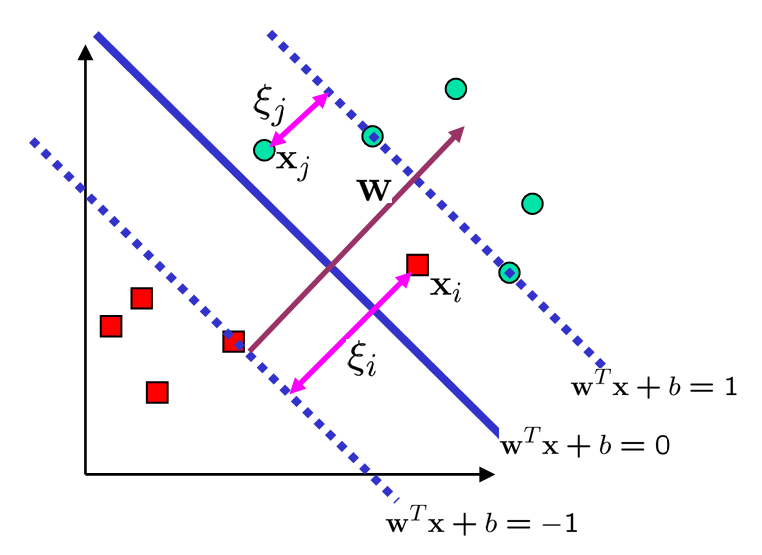
\includegraphics[scale=0.5]{SVM-SoftMargin}
	\caption{مسئله حاشیه نرم در ماشین بردار پشتیبان}
	\label{fig:SVM-SM}
\end{figure}

\begin{equation}
\begin{split}
\min_{w} \quad &\frac{1}{2}{{\left\| w \right\|}^{2}}+C\sum\limits_{i=1}^{n}{{{\xi }_{i}}} \\
\textrm{\lr{s.t. }}  \quad &{{y}_{i}}({{w}^{T}}{{x}_{i}}+b)\text{ }+{{\xi }_{i}}\ge 1,\forall i
\end{split}
\label{eq:9}
\end{equation}
در رابطه \ref{eq:9}، متغیر $\xi _{i}\ge 0$ خطای متناظر برای هر نمونه  $x_i$ است. پارامتر $C$ بیانگر تعادل بین بیشینه کردن حاشیه و خطای دسته‌بندی است. مقدار این پارامتر قبل از آموزش دسته‌بند باید مشخص گردد. مانند مسئله حاشیه سخت، برای حل کردن مسئله اصلی  از تابع لاگرانژ استفاده می‌شود که در رابطه زیر تعریف شده است.
\begin{equation}
L(w,b,\xi, \alpha, \beta )=\frac{1}{2}{{\left\| w \right\|}^{2}} + C\sum\limits_{i=1}^{m}{{{\xi }_{i}}}  -\sum\limits_{i=1}^{m}{{{\alpha }_{i}}({{y}_{i}}({{w}^{T}}{{x}_{i}}+b)-1 + \xi_{i} }) - \sum\limits_{i=1}^{m}{\beta_{i}\xi_{i}}
\label{eq:10}
\end{equation}
در رابطه \ref{eq:10}، بردار $\alpha$  و $\beta$  ضرایب لاگرانژ هستند. برای حل کردن رابطه \ref{eq:10}، نسبت به  $w$، $b$ و $\xi$  مشتق می‌گیریم.
\begin{align}
\label{eq:11}
\begin{split}
\frac{\partial L}{\partial b}&=0\quad \Rightarrow \quad \sum\limits_{i=1}^{m}{{{\alpha }_{i}}{{y}_{i}}}=0
\end{split}\\ 
\label{eq:12}
\begin{split}
\frac{\partial L}{\partial w}&=0 \quad \Rightarrow \quad w = \sum\limits_{i=1}^{m}{\alpha_{i}y_{i}x_{i}}.
\end{split}\\
\label{eq:13}
\begin{split}
\frac{\partial L}{\partial \xi}&=0 \quad \Rightarrow \quad \alpha_{i} + \beta_{i} = C
\end{split}  
\end{align}
با در نظر گرفتن روابط بالا، مسئله دوگان برای حالت حاشیه نرم به صورت زیر تعریف می‌شود.
\begin{equation}
\begin{split} 
\min\limits_{\alpha} \quad &\frac{1}{2}\sum\limits_{i=1}^{m}{\sum\limits_{j=1}^{m}{{{\alpha }_{i}}{{\alpha }_{j}}{{y}_{i}}{{y}_{j}}x_{i}^{T}{{x}_{j}}-\sum\limits_{k=1}^{m}{{{\alpha }_{k}}}}} \\
\textrm{\lr{s.t. }} \quad &\sum\limits_{i=1}^{m}{\alpha_{i}y_{i}}=0, \\
&0 \le \alpha_{i}\le C,\text{ }\forall i
\end{split}
\label{eq:14}
\end{equation}
\indent راه حل مسئله \ref{eq:14} شبیه به مسئله \ref{eq:5} در حالت حاشیه سخت است. با این تفاوت که برای ضرایب لاگرانژ یک حد بین صفر تا پارامتر  تعریف شده است. پارامتر  انعطاف‌پذیری دسته‌بند را افزایش می‌دهد. مقدار این پارامتر با داشتن دانش قبلی از مسئله و یا جستجوی شبکه‌ای تعیین می‌شود. همانطور که در شکل ‏\ref{fig:SVM-SM} نشان داده شده است، بردارهای پشتیبان لزوما روی خط حاشیه قرار ندارند. در مسئله حاشیه نرم، تابع تصمیم مشابه حالت حاشیه سخت به صورت زیر تعریف می‌شود.
\begin{equation}
D(x)=sign({{w}^{T}}x+b) = sign(\sum\limits_{i \in S}{\alpha_{i}y_{i}x_{i}^{T}} x + b)
\label{eq:15}
\end{equation}
در رابطه \ref{eq:15}، مجموعه $S$ نشان دهنده بردارهای پشتیبان است.

\subsection{ماشین بردار پشتیبان با هسته غیر خطی}\label{sec:2:1:3}
در مسائل حاشیه سخت و نرم، فرض گرفته می‌شود که نمونه‌ها در فضای ورودی به صورت خطی جدا پذیر هستند. با این حال در مواردی که نمونه‌ها به صورت خطی جدا پذیر نیستند، نمونه‌ها $x_i$ به فضای ویژگی\footnote{\lr{Feature space}}  با ابعاد بیشتر با تکنیک حقه‌ی هسته\footnote{\lr{Kernel trick}}  نگاشت می‌شود. در این فضا، ماشین بردار پشتیبان یک ابرصفحه جدا کننده بهینه برای جداسازی نمونه‌ها پیدا می‌کند. شکل \ref{fig:SVM-Ker} تکنیک حقه‌ی هسته را نشان می‌دهد.

\begin{figure}[!t]
	\centering
	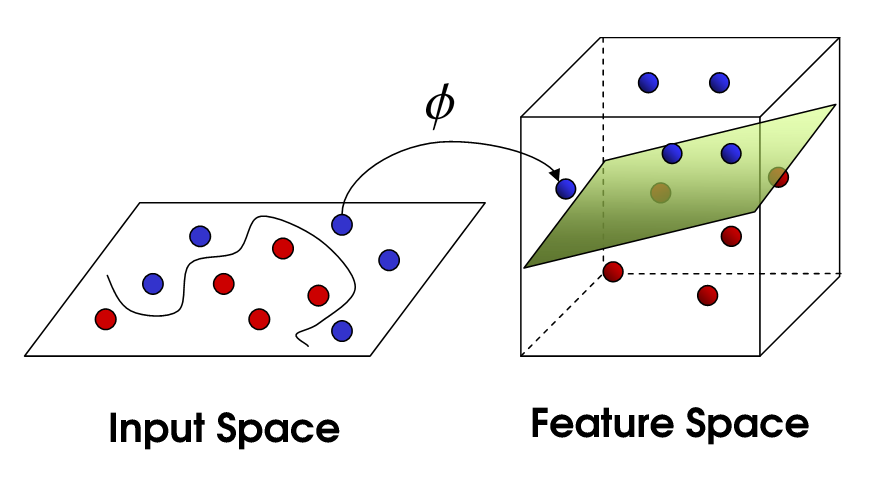
\includegraphics[scale=0.4]{SVM-Kernel}
	\caption{نگاشت نمونه‌ها با تکنیک حقه‌ی هسته}
	\label{fig:SVM-Ker}
\end{figure}

در نسخه غیر خطی ماشین بردار پشتیبان، مسئله \ref{eq:14} به صورت زیر تعریف می‌شود.
\begin{equation}
\begin{split} 
\min\limits_{\alpha} \quad &\frac{1}{2}\sum\limits_{i=1}^{m}{\sum\limits_{j=1}^{m}{{{\alpha }_{i}}{{\alpha }_{j}}{{y}_{i}}{{y}_{j}}K(x_{i},{{x}_{j}})-\sum\limits_{k=1}^{m}{{{\alpha }_{k}}}}} \\
\textrm{\lr{s.t. }} \quad &\sum\limits_{i=1}^{m}{\alpha_{i}y_{i}}=0, \\
&0 \le \alpha_{i}\le C,\text{ }\forall i
\end{split}
\label{eq:16}
\end{equation}
در رابطه \ref{eq:16}‏، تابع هسته  $K({{x}_{i}},{{x}_{j}})$ نمونه‌ها را به فضای ویژگی نگاشت می‌کند. تابع‌های هسته متداول شامل  \lr{RBF}\footnote{\lr{Radial basis function (RBF)}}، چند جمله‌ای و سیگموئید\footnote{\lr{Sigmoid}}  هستند. تابع تصمیم در نسخه غیر خطی به صورت زیر تعریف می‌شود.
\begin{equation}
D(x)= sign(\sum\limits_{i \in S}{\alpha_{i}y_{i}}K(x_{i}, x) + b)
\label{eq:17}
\end{equation}

\subsection{پیشینه پژوهش در ماشین بردار پشتیبان}\label{sec:2:1:4}
ماشین بردار پشتیبان بنیان ریاضی قوی‌ای دارد و دارای قدرت تعمیم‌پذیری بالایی است. از این رو در مسائل مختلف انند تشخیص آریتمی‌های قلبی \cite{nasiri2009}، شناسایی نفوذ به شبکه‌های کامپیوتری \cite{raman2017}، دسته‌بندی متن\cite{lee2012} و شناسایی 
هرزنامه \cite{zoubi2018} مورد استفاده قرار گرفته است. با این حال ماشین بردار پشتیبان نقاط ضعفی نیز دارد که مهم‌ترین آن‌ها عبارتند از:
\begin{enumerate}
	\item ماشین بردار پشتیبان برای بدست آوردن ابرصفحه بهینه یک مسئله بهینه‌سازی از نوع برنامه‌ریزی درجه دو حل می‌کند. مرتبه زمانی حل کردن چنین مسئله‌ای برابر با   $\mathcal{O}({{m}^{3}})$ است.  $m$ تعداد نمونه‌های آموزشی می‌باشد. این مرتبه زمانی، آموزش روش ماشین بردار پشتیبان را برای مجموعه داده‌های بزرگ به طور قابل توجه‌ای کند می‌کند.
	\item در روش \lr{SVM}، بردارهای پشتیبان نقش مهمی در ایجاد مدل دارند. در صورتی که این بردارها از نمونه‌های پرت یا نویزی باشد، دقت و تعمیم‌پذیری مدل خروجی کاهش می‌یابد. در نتیجه روش \lr{SVM} به نمونه‌های پرت و نویزی حساس است.
	\item چنانچه نمونه‌های یک کلاس از کلاس دیگر بسیار بیشتر باشد (مجموعه داده نامتوازن باشد.)، مدل ایجاد شده توسط  \lr{SVM} به سمت کلاس اکثریت گرایش پیدا می‌کند. در نتیجه مدل در تشخیص کلاس اقلیت ناتوان است.
\end{enumerate}

\indent در دو دهه اخیر، روش‌های یادگیری جدیدی مبتنی \lr{SVM} ارائه شده است که برخی از آن‌ها نقاط ضعف بالا را حل می‌کند. در سال 1999، ماشین بردار پشتیبان کمترین مربعات\footnote{\lr{Least squares support vector machines  (LS-SVM)}}  ارائه شد \cite{suykens1999}. در این روش قید در مسئله بهینه‌سازی از نامساوی به مساوی تبدیل شده است. بطوریکه به جای حل کردن مسئله بهینه‌سازی از نوع برنامه‌ریزی درجه دو، دستگاه معادلات خطی حل می‌گردد. در نتیجه سرعت یادگیری برای مجموعه داده‌های بزرگ بسیار بیشتر می‌شود و نقطه ضعف مورد اول تا حد زیادی حل شده است.

در سال 2001، ماشین بردار پشتیبان مبتنی بر مفهوم نزدیکی\footnote{\lr{Proximal Support Vector Machine (PSVM)}}  (\lr{PSVM}) ارائه شد \cite{mang2001}. در این روش دو ابرصفحه موازی برای دسته‌بندی نمونه‌ها ایجاد می‌شود. در سال 2002، ماشین بردار پشتیبان فازی\footnote{\lr{Fuzzy Support Vector Machine (FSVM)}}  (\lr{FSVM}) \cite{lin2002} ارائه گردید. در این روش به هر یک از نمونه‌های هر دو کلاس، تعلق فازی داده می‌شود. بطوریکه اثر نمونه‌های نویزی و پرت در ایجاد مدل خروجی کم خواهد شد. در سال 2006، ماشین بردار پشتیبان با رویکرد مقدار ویژه تعمیم یافته\footnote{\lr{Generalized Eigenvalue Proximal Support Vector Machine (GEPSVM)}}  (\lr{GEPSVM}) ارائه شد \cite{mang2006}. برخلاف روش \lr{PSVM}، این روش دو ابرصفحه غیر موازی ایجاد می‌کند که هر یک از این ابرصفحه‌ها به نمونه‌های کلاس خود نزدیک است و از نمونه‌های کلاس مقابل تا جای ممکن فاصله می‌گیرد. همچنین روش \lr{PSVM} بر روی مسئله \lr{XOR} عملکرد بهتری نسبت به روش \lr{SVM} اصلی دارد.

در سال 2007، ماشین بردار پشتیبان دو قلو\footnote{\lr{Twin Support Vector Machine (TSVM)}}  (\lr{TSVM}) با هدف بهبود پیچیدگی زمانی \lr{SVM} ارائه گردید \cite{jayadeva2007}. ایده اصلی این روش یادگیری، بدست آوردن دو ابرصفحه غیر موازی است. بطوریکه هر ابرصفحه غیر موازی به نمونه‌های کلاس خود نزدیک است و نمونه‌های کلاس مقابل دور می‌شود. دو مسئله بهینه‌سازی کوچک از نوع برنامه‌ریزی درجه دو برای بدست آوردن این دو ابرصفحه غیر موازی حل می‌گردد. در حالی‌که در روش \lr{SVM} یک مسئله بهینه‌سازی بزرگ حل می‌شود. در نتیجه، روش ماشین بردار پشتیبان دو قلو در تئوری 4 برابر سریعتر از روش \lr{SVM} است. در بخش ‏2-2 ماشین بردار پشتیبان دو قلو و پیشینه پژوهش آن به طور کامل بررسی می‌شود.

در سال‌های اخیر نیز، روش‌های جدید مبتنی بر \lr{SVM} ارائه شده است. در سال 2018، می‌توان به روش یادگیری برخط مبتنی بر بدترین نمونه‌ی نقض‌کننده\footnote{\lr{Online Learning Algorithm using Worst-Violators (OLLAWV)}}  اشاره کرد \cite{melki2018}. این الگوریتم بر اساس گرادیان نزولی تصادفی\footnote{\lr{Stochastic Gradient Descent (SGD)}}  طراحی شده است و مسئله اصلی در روش \lr{SVM} را به جای مسئله دوگان حل می‌کند. مزایای این روش، دقت بهتر، سرعت یادگیری بیشتر برای مجموعه داده‌های بزرگ و همچنین مدل خلوت\footnote{\lr{Sparse}}  می‌باشد.

\section{ماشین بردار پشتیبان دو قلو}\label{sec:2:2}
در این بخش، ابتدا نسخه خطی ماشین بردار پشتیبان دو قلو شرح داده می شود. سپس نسخه غیر خطی این روش توضیح داده شده و در آخر پیشینه پژوهش آن و روش‌های مبتنی بر \lr{TSVM} بررسی می‌شود.

\subsection{ماشین بردار پشتیبان دو قلو خطی}\label{sec:2:2:1}
ایده اصلی روش \lr{TSVM}، ایجاد دو ابرصفحه غیر موازی است \cite{jayadeva2007}. بطوریکه هر ابرصفحه غیر موازی از نمونه‌های کلاس خود کمترین فاصله را دارد و از نمونه‌های کلاس مقابل حداکثر فاصله ممکن را خواهد داشت. برای تشریح بهتر این روش، یک مسئله دسته‌بندی دوکلاسه با $m_1$  نمونه آموزشی کلاس مثبت و  $m_2$ نمونه آموزشی کلاس منفی را در نظر می‌گیریم. همچنین فرض می‌کنیم که ماتریس   $A\in {{\mathbb{R}}^{{{m}_{1}}\times n}}$ بیانگر نمونه‌های کلاس مثبت و ماتریس  $B\in {{\mathbb{R}}^{{{m}_{2}}\times n}}$ بیانگر نمونه‌های کلاس منفی است. روش \lr{TSVM} در حالت خطی به دنبال دو ابرصفحه غیر موازی در فضای  ${{\mathbb{R}}^{n}}$ است که در رابطه زیر تعریف شده است.
\begin{equation}
{{x}^T}{{w}_{1}}+{{b}_{1}}=0 \quad \textrm{\lr{and }} \quad {{x}^T}{{w}_{2}}+{{b}_{2}}=0
\label{eq:18}
\end{equation}
در رابطه \ref{eq:18}،  ${{w}^{(1)}},{{w}^{(2)}}\in {{\mathbb{R}}^{n}}$ نشان دهنده مختصات دو ابرصفحه و  ${{b}^{(1)}},{{b}^{(2)}}\in {\mathbb{R}}$ نشان دهنده بایاس است. شکل ‏2 4 تفسیر هندسی روش ماشین بردار پشتیبان دوقلو خطی را نشان می‌دهد. در روش \lr{TSVM}، دو مسئله بهینه‌سازی از نوع برنامه‌ریزی درجه دو برای بدست آوردن دو ابرصفحه غیر موازی به صورت زیر تعریف می‌شود.
\begin{figure}[!t]
	\centering
	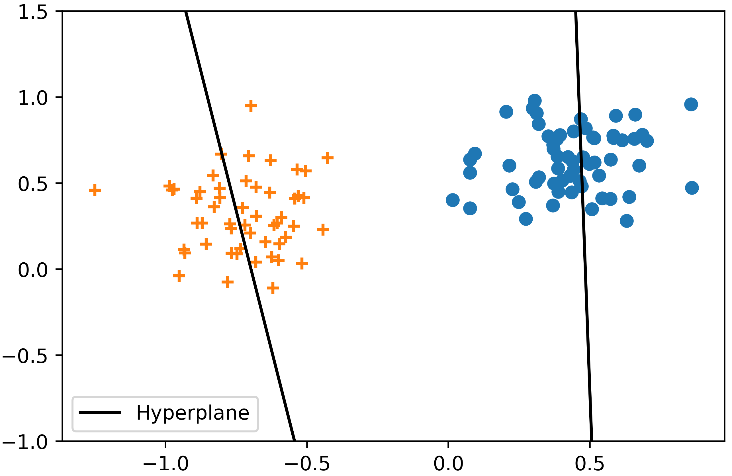
\includegraphics[scale=0.75]{TSVM-idea}
	\caption{تفسیر هندسی روش ماشین بردار پشتیبان دو قلو خطی}
	\label{fig:TSVM-idea}
\end{figure}
\begin{align}
\label{eq:19}
\begin{split}
\underset{{{w}_{(1)}},{{b}_{(1)}}}{\mathop{min}}\,\qquad  & \frac{1}{2}{{\left\| A{{w}^{(1)}}+{{e}_{1}}{{b}^{(1)}} \right\|}^{2}}+{{C}_{1}}e_{2}^{T}{{y}_{2}}  \\
\text{\lr{s.t.}} \qquad  & -(B{{w}^{(1)}}+{{e}_{2}}{{b}^{(1)}})+{{y}_{2}}\ge {{e}_{2}}\text{ },{{y}_{2}}\ge 0  
\end{split} \\
%\end{equation}
%\begin{equation}
\label{eq:20}
\begin{split}
\underset{{{w}_{(2)}},{{b}_{(2)}}}{\mathop{min}}\,\qquad  & \frac{1}{2}{{\left\| B{{w}^{(2)}}+{{e}_{2}}{{b}^{(2)}} \right\|}^{2}}+{{C}_{2}}e_{1}^{T}{{y}_{1}}  \\
\text{\lr{s.t.}} \qquad  & (A{{w}^{(2)}}+{{e}_{1}}{{b}^{(2)}})+{{y}_{1}}\ge {{e}_{1}}\text{ },{{y}_{1}}\ge 0  
\end{split}
\end{align}
\bigbreak
در روابط \ref{eq:19} و \ref{eq:20}،  $C_1$ و $C_2$  پارامترهای خطا،  $e_1$ و  $e_2$ بردار با درایه‌های یک در ابعاد متناسب،  $y_1$ و $y_2$  متغیر کمکی هستند. لازم به ذکر است که تعداد نمونه‌ها در مسائل بهینه‌سازی روش \lr{TSVM} تقریبا برابر با $m/2$ در نظر گرفته می‌شود. با این حال در روش \lr{SVM}، در قید مسئله بهینه‌سازی تمام نمونه‌های آموزشی نقش دارند. بنابراین زمان اجرای روش \lr{TSVM} از روش \lr{SVM} حدود 4 برابر سریع‌تر است که زیر نشان داده شده است.
\begin{equation}
\Big[({{m}^{3}})/(2\times {{(\frac{m}{2})}^{3}})\Big] = 4.
\label{eq:21}
\end{equation}

مانند روش \lr{SVM}، برای حل کردن مسائل بهینه‌سازی \ref{eq:19}، از تابع لاگرانژ استفاده می‌کنیم.
\begin{equation}
\begin{split}
L(w_{1},b_{1},y_{2}, \alpha, \beta )= &\frac{1}{2}(A{{w}^{(1)}}+{{e}_{1}}{{b}^{(1)}})^{T}(A{{w}^{(1)}}+{{e}_{1}}{{b}^{(1)}}) + {{C}_{1}}e_{2}^{T}y_{2} \\
&-\alpha^{T}(-(Bw^{(1)}+e_{2}b^{(1)})+y_{2} - e_{2}) - \beta^{T}y_{2}
\end{split}
\label{eq:22}
\end{equation}

در رابطه \ref{eq:22}، $\alpha=(\alpha_{1}, \alpha_{2}, \dots,\alpha_{m_{2}})^{T}$ و $\beta=(\beta_{1}, \beta_{2}, \dots,\beta_{m_{2}})^{T}$ بردارهای ضرایب لاگرانژ هستند.  با مشتق‌گیری از رابطه \ref{eq:22}، شرایط \lr{KKT}\footnote{\lr{Karush-Kuhn-Tucker}}  زیر برقرار می‌شود.
\begin{align}
\label{eq:23}
\begin{split}
A^{T}(A{{w}^{(1)}}+{{e}_{1}}{{b}^{(1)}}) + B^{T}\alpha = 0.
\end{split} \\
\label{eq:24}
\begin{split}
e_{1}^{T}(A{{w}^{(1)}}+{{e}_{1}}{{b}^{(1)}}) + e_{2}^{T}\alpha = 0.
\end{split}\\
\label{eq:25}
\begin{split}
C_{1}e_{2} - \alpha - \beta = 0.
\end{split} 
\end{align}
با توجه اینکه $\beta \ge 0$، از رابطه \ref{eq:25} خواهیم داشت:
\begin{equation}
0 \le \alpha \le {C}_{1}
\label{eq:26}
\end{equation}

سپس با ترکیب کردن \ref{eq:23} و \ref{eq:24}، رابطه زیر بدست می‌آید.
\begin{equation}
[A^{T}\ e^{T}_{1}][A\ e_{1}][w^{(1)}\ b^{(1)}]^{T} + [B^{T}\ e^{T}_{2}]\alpha = 0.
\label{eq:27}
\end{equation}

با تعریف کردن ماتریس $H$ و $G$ به صورت $H=[A\text{ }e]$ و $G=[B\text{ }e]$، رابطه \ref{eq:27} به صورت زیر بازنویسی می‌شود.
\begin{equation}
\left[ \begin{aligned}
& {{w}^{(1)}} \\
& {{b}^{(1)}} \\
\end{aligned} \right]= -{{({{H}^{T}}H)}^{-1}}{{G}^{T}}\alpha
\end{equation}
